\documentclass[11pt,a4paper]{article}
\usepackage[utf8]{inputenc}
\usepackage[german]{babel}
\usepackage{amsmath}
\usepackage{amsfonts}
\usepackage{subfig}
\usepackage{amssymb}
\usepackage{siunitx,physics}
\usepackage{mathtools}
\usepackage{graphicx}
%\usepackage{Here}
\usepackage[version=4]{mhchem}
\usepackage{url}
\usepackage{setspace}
\usepackage[left=2.5cm,right=2.5cm,top=2.5cm,bottom=2cm]{geometry}
[biblography=totocnumbered]
\usepackage{fancyhdr}
\usepackage{scrextend}
\usepackage{hyperref}
\pagenumbering{gobble}

\makeatletter
\newcommand\bigcdot{\mathpalette\bigcdot@{.5}}
\newcommand\bigcdot@[2]{\mathbin{\vcenter{\hbox{\scalebox{#2}{$\m@th#1\bullet$}}}}}
\makeatother

\makeatletter
%\renewcommand*\bib@heading{%
%  \subsection*{}%
%  \@mkboth{\refname}{\refname}}
%\makeatother
\numberwithin{equation}{section}
\numberwithin{figure}{section}

\renewcommand{\labelitemii}{\labelitemfont$\vartriangleright$}
\begin{document}\\
\begin{addmargin}[25pt]{0pt}
Biologische Materialien sind häufig in einer hierarchischen Struktur aufgebaut, siehe Abbildung \ref{fig:hierarchie}. Die hierarchische Struktur sorgt dafür, dass sich Risse schlechter ausbreiten können und sich die Spannung gut verteilt und so kein Bereich zu stark belastet wird. In der hierarchischen Struktur gilt: je mehr hierarchische Levels vorhanden sind umso höher ist die Steifigkeit und die Zähigkeit des Kompositmaterials \\
\begin{figure}[h]
    \centering
    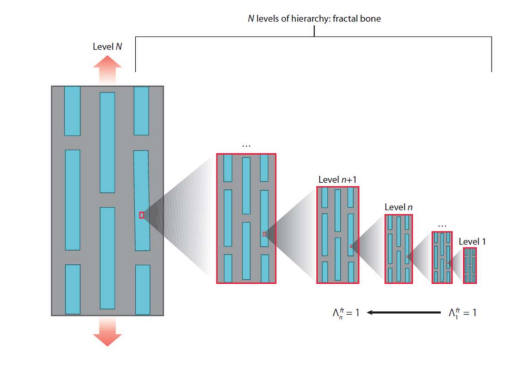
\includegraphics[scale = 0.85]{images/Materialwissenschaften/hierarchische_struktur.png}
    \caption{Hierarchische Struktur in biologischen Materialien}
    \label{fig:hierarchie}
\end{figure}
\end{addmargin}

\end{document}